\documentclass[tikz,border=8pt]{standalone}
% Shared look for every TikZ diagram. Load with \input{../../tools/tikz-style.tex}
\usepackage[T1]{fontenc}
\usepackage{lmodern}
\renewcommand{\sfdefault}{lmr}  % diagrams use the same serif as the text
\usetikzlibrary{arrows.meta, positioning, shapes.geometric, calc, fit, backgrounds}
\definecolor{cblue}{HTML}{4C78A8}
\definecolor{corange}{HTML}{F58518}
\definecolor{cgreen}{HTML}{54A24B}
\definecolor{cred}{HTML}{E45756}
\definecolor{cpurple}{HTML}{B279A2}
\definecolor{cgrey}{HTML}{6B6B6B}
\tikzset{
  every picture/.style={font=\sffamily, line width=1.2pt},
  box/.style={draw=#1, fill=#1!12, rounded corners=4pt, align=center, inner sep=7pt, minimum height=1.1cm},
  box/.default=cgrey,
  arrow/.style={-{Stealth[length=3mm]}, draw=cgrey, line width=1.4pt},
  title/.style={font=\sffamily\bfseries\Large},
  note/.style={font=\sffamily\small, text=cgrey, align=center},
}
\AtBeginDocument{\hyphenpenalty=10000 \exhyphenpenalty=10000}

\begin{document}
\begin{tikzpicture}[every node/.append style={font=\sffamily\large}]
% one panel: #1 x-offset; rows = die 1 (1 top .. 6 bottom), columns = die 2
\newcommand{\cell}[4]{\fill[#4] ({#1+#3-1},{-#2}) rectangle ++(1,1);}
% ---------- left: independent ----------
\begin{scope}
  \foreach \r in {1,...,6} {\cell{0}{\r}{6}{cblue!35}}
  \foreach \c in {1,...,6} {\cell{0}{3}{\c}{corange!35}}
  \cell{0}{3}{6}{cpurple!70}
  \draw[cgrey, line width=0.6pt] (0,-6) grid (6,0);
  \foreach \k in {1,...,6} {\node at (\k-0.5,0.45) {\k}; \node at (-0.45,-\k+0.5) {\k};}
  \node[font=\sffamily] at (3,1.15) {die 2};
  \node[font=\sffamily, rotate=90] at (-1.2,-3) {die 1};
  \node[title, text=cblue] at (3,2.2) {independent};
  \node[align=left, anchor=north west] at (-0.6,-6.4) {
    {\color{cblue}$A$: die 2 = 6} \quad {\color{corange}$B$: die 1 = 3}\\[2pt]
    $P(A \cap B) = \tfrac{1}{36} = \tfrac{1}{6}\times\tfrac{1}{6}$\\[2pt]
    inside row $B$, $A$ is 1 of 6 cells};
\end{scope}
% ---------- right: dependent ----------
\begin{scope}[xshift=9.6cm]
  \foreach \c in {1,...,6} {\cell{0}{6}{\c}{corange!35}}
  \foreach \r/\c in {4/6,5/5,5/6,6/4,6/5,6/6} {\cell{0}{\r}{\c}{cred!45}}
  \foreach \c in {4,5,6} {\cell{0}{6}{\c}{cpurple!70}}
  \draw[cgrey, line width=0.6pt] (0,-6) grid (6,0);
  \foreach \k in {1,...,6} {\node at (\k-0.5,0.45) {\k}; \node at (-0.45,-\k+0.5) {\k};}
  \node[font=\sffamily] at (3,1.15) {die 2};
  \node[title, text=cred] at (3,2.2) {not independent};
  \node[align=left, anchor=north west] at (-0.6,-6.4) {
    {\color{cred}$C$: sum $\geq$ 10} \quad {\color{corange}$D$: die 1 = 6}\\[2pt]
    $P(C \cap D) = \tfrac{3}{36} \neq \tfrac{1}{6}\times\tfrac{1}{6}$\\[2pt]
    inside row $D$, $C$ is 3 of 6 cells};
\end{scope}
\end{tikzpicture}
\end{document}
